


\tikzset{every picture/.style={line width=0.75pt}} %set default line width to 0.75pt        

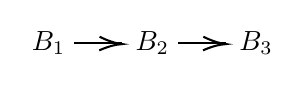
\begin{tikzpicture}[x=0.75pt,y=0.75pt,yscale=-1,xscale=1]
%uncomment if require: \path (0,797); %set diagram left start at 0, and has height of 797


% Text Node
\draw (380,0) node [anchor=north west][inner sep=0.75pt]    {$B_{1}$};
% Text Node
\onslide<4->{\draw (430,0) node [anchor=north west][inner sep=0.75pt]    {$B_{2}$};}
% Text Node
\onslide<5->{\draw (480,0) node [anchor=north west][inner sep=0.75pt]    {$B_{3}$};}
% Connection
\onslide<4->{\draw    (402,7) -- (425,7) ;
\draw [shift={(425,7.4)}, rotate = 181.36] [color={rgb, 255:red, 0; green, 0; blue, 0 }  ][line width=0.75]    (10.93,-3.29) .. controls (6.95,-1.4) and (3.31,-0.3) .. (0,0) .. controls (3.31,0.3) and (6.95,1.4) .. (10.93,3.29)   ;}
% Connection
\onslide<5->{\draw    (452,7) -- (475,7) ;
\draw [shift={(475,7.4)}, rotate = 181.4] [color={rgb, 255:red, 0; green, 0; blue, 0 }  ][line width=0.75]    (10.93,-3.29) .. controls (6.95,-1.4) and (3.31,-0.3) .. (0,0) .. controls (3.31,0.3) and (6.95,1.4) .. (10.93,3.29)   ;}

\end{tikzpicture}
